\documentclass{article}
\usepackage{amsmath}
\usepackage{amsfonts}
\usepackage{amssymb}
\usepackage{booktabs}
\usepackage{graphicx}
\usepackage[margin=1in]{geometry}
\usepackage{hyperref}

\title{Ex1 Writeup}
\author{}
\date{}

\begin{document}

\begin{flushright}
    \textbf{\small Yujia Zhang \\
    \today}
\end{flushright}

\begin{center}
    \textbf{\large Exercise Solution}
\end{center}

\begin{flushleft}
\vspace{0.3cm}

{\itshape
\textbf{Summary:} Predicting exact home and away corners is hard, so the model should not stop at point forecasts. The useful step is to turn home and away means, variances, and market-aware calibration into a betting distribution.

\par\vspace{0.25cm}

Once that distribution is believable, Kelly can compound capital even under realistic fees and stake caps, but full Kelly is too aggressive in practice. Fractional Kelly is more sensible because it gives a better Sharpe-ratio-like risk-adjusted profile, which matters more here than maximising terminal cash.

\par\vspace{0.25cm}

Questions 2 and 3 are standard at the formula level: EV, distributions, and Kelly are well known. The real issue is whether the model probabilities behind those formulas are believable. That is why the assumptions have to be checked, especially with Monte Carlo. If the EV is not credible, Kelly is not credible either, and because Kelly is highly sensitive to probability error, stress testing is not optional.

}

\vspace{0.45cm}
\end{flushleft}

\noindent \textbf{Question 1. Build a predictive model for the number of home and away corners. Explain the process -
including data exploration, features and model selection/comparison, model validation etc?}

\noindent \textbf{Answer.} The Q1 path is:
\[
\texttt{data\_cleaning.ipynb}
\rightarrow
\texttt{q1\_pipeline.py}
\]
Inside \texttt{q1\_pipeline.py}, two sub-modules are fitted: \texttt{team\_strength.py} and \texttt{team\_variance.py}. The execution order is:
\begin{enumerate}
    \item \texttt{data\_cleaning.ipynb} does the data preprocessing.
    \item \texttt{q1\_pipeline.py} loads those parquet files and builds the full Q1 dataset.
    \item Stage 1a in \texttt{q1\_pipeline.py} calls \texttt{team\_strength.py} to build leak-free pre-match team strength features.
    \item Stage 1b builds rolling recent-form features from earlier matches only.
    \item Stage 2 fits the mean models for home corners and away corners.
    \item Stage 3 calls \texttt{team\_variance.py} to estimate conditional variance, then applies the late-window correction, market-teacher adjustment (no odds are used in this stage), and residual quantile calibration.
\end{enumerate}
So \texttt{q1\_pipeline.py} is the orchestrator, while \texttt{team\_strength.py} and \texttt{team\_variance.py} are helper modules that produce two of the most important feature blocks.

\bigskip

\noindent \textbf{Data exploration:}

\noindent See \texttt{data\_cleaning.ipynb}. The exploration step is simple but important: first check row counts, date ranges, duplicate match keys, impossible values, and missing coverage across the raw match and price tables. Then the cleaning pass removes the obvious bad rows: the corner outlier value \(999\), conflicting records, duplicate rows after the first occurrence, odds below \(1\) for \texttt{oh}/\texttt{oa}, and negative \texttt{od} values inside the OU and 1X2 tables. After that, 7 teams still have missing corner history in the raw match file, so those match identities are repaired by matching against the price tables. The market odds themselves are not used as features at this stage; they are only used to recover the missing match records. The cleaned outputs are written to \texttt{train.parquet}, \texttt{betting.parquet}, and \texttt{all\_matches.parquet}.\\

\noindent \textbf{Train / validation / test split:}

\noindent The split is fully time ordered.
\begin{itemize}
    \item Q1 model window: \(11{,}198\) matches from 2020-08-08 to 2024-12-08.
    \item Q1 train split: \(8{,}956\) matches from 2020-08-08 to 2023-10-21.
    \item Q1 validation split: \(2{,}242\) matches from 2023-10-21 to 2024-12-08.
    \item Betting holdout window: \(1{,}911\) matches from 2024-08-09 to 2025-05-11.
    \item Betting partition A: \(764\) matches from 2024-08-09 to 2024-12-14 15:00.
    \item Betting partition B: \(1{,}147\) matches from 2024-12-14 15:15 to 2025-05-11.
\end{itemize}
The point of this layout is to keep the roles separate. The Q1 mean model is fitted on the historical train block and checked on a later validation block. The later betting window is never used to fit the mean head. Inside that betting window, partition A is only for calibration and threshold tuning, and partition B is reserved for the final out-of-sample betting evaluation.


\noindent \textbf{What does Q1 actually predict for one match, and where do mean and variance enter?}

\noindent Q1 makes two different kinds of prediction for each match.
\begin{enumerate}
    \item A \textbf{point forecast}: how many corners the home team is expected to win, and how many corners the away team is expected to win.
    \item An \textbf{uncertainty forecast}: how much those two point forecasts are expected to vary around their centres.
\end{enumerate}

The point forecast is simply the pair
\[
\hat{\mu}_{home}=\texttt{pred\_home\_corners},\qquad
\hat{\mu}_{away}=\texttt{pred\_away\_corners}.
\]
If the model says \(5.8\) and \(4.3\), then Q1's direct answer for that match is ``home about 5.8 corners, away about 4.3 corners.'' The variance does not create a second point forecast and it does not shift the mean. It only says how uncertain the model is around those centres.

After the two means are predicted, I estimate one variance for the home prediction and one variance for the away prediction (later used in Q2). So the final Q1 output is:
\[
\hat{\mu}_{home},\;
\hat{\mu}_{away},\;
\hat{\sigma}^{2}_{home},\;
\hat{\sigma}^{2}_{away},
\]
plus residual quantile anchors \(q10, q50, q90\) that will be also used by Q2.

\bigskip

\noindent \textbf{To predict the number of corners, I introduced a team-strength model as a sub-model of mean prediction, since team strength is a key determinant of corner output.}

\noindent The team-strength block turns raw match history into a running estimate of each team's latent corner profile. It is best described as an \textbf{Elo-style online updater}, but it is not the classical Elo system used for win/loss results.

In classical Elo, each team has one rating and the update is driven by whether the team won or lost. Here, each team carries two hidden states:
\begin{itemize}
    \item an attack rating: how much the team tends to create corners;
    \item a defence leakiness rating: how many corners the team tends to allow.
\end{itemize}
The model walks through matches in chronological order. Before updating anything, it reads the current ratings and builds the features for that match. Only after the match is observed does it update the two teams' ratings. Every row only uses information that was available. There is no look-ahead leakage.

The core abstraction is:
\[
\log(\lambda_{home})
=
\text{league home baseline}
+
\text{home attack}
+
\text{away defensive leakiness},
\]
\[
\log(\lambda_{away})
=
\text{league away baseline}
+
\text{away attack}
+
\text{home defensive leakiness}.
\]
See team\_strength.read\_features. Here \(\lambda_{home}\) and \(\lambda_{away}\) are the expected home and away corner rates before the match starts. After the match ends, the model compares the realised corners with these expected rates on the log scale and nudges the two teams' latent ratings up or down. Teams with little history move faster. Teams with long history move more slowly. That is what the prior-strength and learning-rate terms are doing.

So the Elo idea appears in the mechanics:
\begin{itemize}
    \item keep a running latent rating per team;
    \item compare expectation with what really happened;
    \item update the ratings after each match;
    \item make updates smaller once the rating is supported by more history.
\end{itemize}
What changes is the target being updated. It is not the final match result. It is the team's corner-creation and corner-concession behaviour.

This block exports the following pre-match features:
\begin{itemize}
    \item overall attack rating and overall defensive leakiness for both teams;
    \item home-only and away-only venue splits;
    \item implied home and away log corner rates;
    \item overall strength difference;
    \item venue-adjusted strength difference.
\end{itemize}
The block answers: how strong is each team at winning corners, how weak is it at preventing them.

\bigskip

\noindent \textbf{How the variance model is fitted.}
The idea is simple: after Q1 makes a point prediction \(\hat{\mu}\) for a match, how far off was it?
The answer is the squared error \((y - \hat{\mu})^{2}\).
A larger squared error means the prediction was further from reality---i.e.\ the match was harder to predict.

The variance model asks: \emph{before} a match is played, can we tell from observable signals whether the prediction will be more or less reliable?
Three signals are used:
\begin{itemize}
  \item the predicted corner count \(\hat{\mu}\) itself---matches expected to produce many corners also tend to be noisier;
  \item market certainty: how one-sided the market price looks, measured as \(\lvert p_{home} - 0.5 \rvert\), where \(p_{home}\) is the no-vig implied probability of the home team winning more corners from the 1X2 market (normalized probability from market odds). A value near zero means the market sees the match as a coin flip; a value near 0.5 means the market is very confident in one side. A more certain market signals a more predictable match, so the prediction error should be smaller;
  \item how erratic that team has been recently (rolling standard deviation)---a team swinging between 3 and 11 corners week to week is genuinely harder to predict.
\end{itemize}

Because squared errors are always positive and heavily skewed, the model takes \(\log\) of them before fitting.
A standard linear regression (OLS) is then run with those three signals as inputs and the log squared error as the output.
The predicted log error is converted back to a variance by exponentiating.
One final multiplicative correction is applied so that the average predicted variance exactly matches the average realised squared error on the training data---this keeps the model honest on the overall scale.
Home and away corners each get their own separate variance model.

\medskip
\noindent \textbf{How the quantile model is fitted.}
The quantile layer answers a different question: not ``how wide is the uncertainty on average?'' but ``given what this specific match looks like, where would the low and high ends of the prediction be?''

Rather than fitting a formula, the approach is a lookup table built from history.
The calibration matches are grouped into cells based on four features: how large the predicted mean is, how volatile the team has been recently, how wide the market spread is, and a composite market certainty score.
The composite certainty is the average of three components:
\begin{itemize}
  \item \(\lvert p_{\text{OU,over}} - 0.5 \rvert\): the OU market quotes a line, e.g.\ ``total corners over/under 9.5''. After removing the bookmaker margin, the implied probability of going over becomes \(p_{\text{OU,over}}\). If the market prices this at \(0.5\), it genuinely sees the match as a coin flip around that line. If it prices it at \(0.8\), it is strongly confident the total will exceed 9.5. The distance from \(0.5\) captures how opinionated the market is about the total corner count.

  \item \(\lvert p_{\text{1X2,home}} - p_{\text{1X2,away}} \rvert\): the 1X2 corner market offers three outcomes---home wins the corner count, away wins it, or they draw. After removing the margin, \(p_{\text{1X2,home}}\) and \(p_{\text{1X2,away}}\) are the implied probabilities for home and away respectively. Their gap measures how dominated the match is: a gap near zero means the market sees the two teams as roughly equal on corners; a large gap means it strongly favours one side.

  \item \(\lvert p_{\text{HC,home}} - 0.5 \rvert\): the handicap market adjusts for expected imbalance by adding or subtracting a fixed number of corners from one team before deciding the winner---for example, home \(-1.5\) means home must win by at least 2 corners to win the bet. After the handicap is applied, \(p_{\text{HC,home}}\) is the implied probability that the home team still wins. A value near \(0.5\) means the handicap has made the match balanced; a value far from \(0.5\) means even the handicapped contest is lopsided, signalling that one team is expected to dominate corners by a wide margin.
\end{itemize}
All probabilities are computed after removing the bookmaker margin (no-vig conversion), so they sum to 1 across each market and reflect the market's genuine belief rather than the raw odds.
Each cell collects all the historical prediction errors (actual minus predicted) for matches that fell into that cell.
The 10th, 50th, and 90th percentiles of those errors are then stored for the cell.

When a new match arrives, it is placed into the matching cell and the stored percentiles are added to its predicted mean to produce the quantile anchors \(\hat{q}_{10}\), \(\hat{q}_{50}\), \(\hat{q}_{90}\).
If no historical matches fell into that cell, the model falls back to the percentiles computed across all matches.
The result is a data-driven description of the prediction tails that makes no assumptions about the shape of the error distribution.

\bigskip

\noindent \textbf{What features go into the corner prediction model? How are they constructed?}

\noindent The final production version uses 28 mean features. They fall into four groups.

\textbf{Group 1: match context.}
\begin{itemize}
    \item \texttt{season\_id}
    \item \texttt{gameweek}
\end{itemize}
These are cheap but useful controls. Season catches slow structural shifts in the data. Gameweek gives the model a simple place to learn season-phase effects.

\textbf{Group 2: team-strength features from Stage 1a.}
\begin{itemize}
    \item \texttt{home\_attack\_rating}
    \item \texttt{home\_defence\_leakiness}
    \item \texttt{away\_attack\_rating}
    \item \texttt{away\_defence\_leakiness}
    \item \texttt{home\_attack\_at\_home}
    \item \texttt{home\_defence\_at\_home}
    \item \texttt{away\_attack\_at\_away}
    \item \texttt{away\_defence\_at\_away}
    \item \texttt{log\_lambda\_home}
    \item \texttt{log\_lambda\_away}
    \item \texttt{strength\_diff}
    \item \texttt{venue\_strength\_diff}
    \item \texttt{league\_log\_baseline\_away}
\end{itemize}
These features summarise the current pre-match corner environment.

\textbf{Group 3: recent corner form.}
\begin{itemize}
    \item exponentially weighted averages of corners won and corners conceded;
    \item rolling-window standard deviations of corners won and conceded.
\end{itemize}
The idea is simple: recent corner flow tells us whether a team is currently producing pressure or absorbing pressure, and recent standard deviation tells us whether that pattern is stable or noisy.

\textbf{Group 4: recent goal state.}
\begin{itemize}
    \item rolling-window goals scored;
    \item rolling-window goals conceded;
    \item rolling-window goal difference.
\end{itemize}
These do not predict corners directly, but they help because style and game state matter. Teams playing on the front foot tend to create different corner profiles from teams sitting deep or chasing games.

For each team row, I record:
\begin{itemize}
    \item \texttt{corners\_for}: corners won by that team in that match;
    \item \texttt{corners\_against}: corners conceded by that team;
    \item \texttt{goals\_for}: goals scored by that team;
    \item \texttt{goals\_against}: goals conceded by that team;
    \item \texttt{goal\_difference}: goals scored minus goals conceded.
\end{itemize}
Then I compute rolling and exponentially weighted summaries using only earlier rows from the same team. That is what keeps this block leak-free.

The 28-feature version keeps Q1 at least as good as the larger model, and it is much better when passed into Q2. That is why I kept 28 and did not drop further.

Top signals are:
\begin{itemize}
    \item \texttt{season\_id}
    \item \texttt{away\_corners\_against\_ewm\_half\_life\_5}
    \item \texttt{home\_goal\_difference\_rolling\_window\_20}
    \item \texttt{home\_corners\_for\_ewm\_half\_life\_5}
    \item \texttt{away\_goal\_difference\_rolling\_window\_20}
\end{itemize}

\bigskip

\noindent \textbf{Why use LightGBM for the mean model instead of Ridge, Random Forest, or XGBoost?}

\noindent Ridge regression is ordinary linear regression with an added penalty on the size of the coefficients: it minimises squared error plus \(\lambda \sum_j \beta_j^2\), where \(\lambda\) controls how much the coefficients are shrunk toward zero.
The shrinkage prevents any single correlated feature from dominating and stops the model from overfitting on noise.
Ridge is a natural first baseline here because corner counts are roughly continuous and in a small numeric range, so a linear model is not obviously wrong, and it can use all 28 features at once without further tuning beyond a single regularisation parameter.
The other candidates---Random Forest, XGBoost, and LightGBM---are all ensemble tree methods that can capture nonlinear interactions, at the cost of more hyperparameters and longer training.

I did not want to claim that by intuition alone, so I ran the comparison in code. On the Q1 validation split:
\begin{center}
\begin{tabular}{lccc}
\toprule
Model & Home MAE & Away MAE & Diff MAE \\
\midrule
LightGBM & 2.2777 & 1.9866 & 3.3489 \\
RandomForest & 2.2866 & 1.9932 & 3.3570 \\
Ridge & 2.2876 & 1.9633 & 3.3346 \\
XGBoost & 2.3194 & 2.0051 & 3.4007 \\
Mean baseline & 2.3906 & 2.0909 & 3.5652 \\
\bottomrule
\end{tabular}
\end{center}

\noindent The baseline is the mean of the training set predictions. It gives:
\begin{itemize}
    \item home MAE \(= 2.3906\);
    \item away MAE \(= 2.0909\);
    \item corner-difference MAE \(= 3.5652\).
\end{itemize}

Here MAE is
\[
\text{MAE}=\frac{1}{n}\sum_{i=1}^{n}\left|y_i-\hat{y}_i\right|.
\]
So home MAE is the average absolute error in predicted home corners, and away MAE is the same quantity for away corners. The best possible value is \(0\). There is no universal finite upper bound in theory, because the target is a nonnegative count and a model can be arbitrarily wrong. In practice the scale is anchored by the observed corner range in this dataset, so a move of about \(0.1\) in MAE is meaningful.

The current 28-feature LightGBM Q1 model gives:
\begin{itemize}
    \item home MAE \(= 2.2777\);
    \item away MAE \(= 1.9866\);
    \item corner-difference MAE \(= 3.3489\).
\end{itemize}

So the gain over baseline is:
\begin{itemize}
    \item home MAE improves by \(0.1129\);
    \item away MAE improves by \(0.1043\);
    \item corner-difference MAE improves by \(0.2163\).
\end{itemize}

That is not a huge jump, but it is real, stable, and achieved without leaking holdout information into the mean head. A useful way to read it is against the practical lower bound in this dataset. For home corners, the irreducible error floor is about \(1.86\), while the constant-mean baseline sits at \(2.39\) and the model brings that down to \(2.28\). So the model removes about \(0.11\) errors per match, out of roughly \(0.53\) errors that were realistically available to remove. For away corners, the floor is about \(1.70\), the baseline is \(2.09\), and the model improves it to \(1.99\), again removing about \(0.10\) errors per match out of roughly \(0.40\) that were realistically available. In plain terms: the model is not close to the theoretical limit, but it is moving in the right direction and doing so consistently. The bigger practical win is that Q1 is not only a slightly better point predictor than the constant mean baseline. It also exports a much richer distributional object that Q2 can actually bet on.

\bigskip

\noindent \textbf{The procedure of prediction:}

\noindent The final prediction is assembled in layers.
\begin{enumerate}
    \item Fit one mean model for home corners and one mean model for away corners. This gives raw point forecasts \(\hat{\mu}_{home}\) and \(\hat{\mu}_{away}\).
    \item Apply the late-window correction to remove recent level bias in the raw mean forecasts.
    \item Apply the market-teacher adjustment. This is trained on partition A and applied out of sample on partition B, so the mean head does not directly read the same market it will later be evaluated against in Q2.
    \item Fit one variance model for the home side and one for the away side. These use predicted mean, market certainty, and rolling volatility to estimate \(\hat{\sigma}^{2}_{home}\) and \(\hat{\sigma}^{2}_{away}\).
    \item Build residual quantiles \(q10, q50, q90\) from historically similar matches. Those quantiles give Q2 a lower anchor, a median anchor, and an upper anchor.
\end{enumerate}

At that point the match-level point forecast is already done:
\[
\text{Q1 point forecast}=(\hat{\mu}_{home}, \hat{\mu}_{away}).
\]
The variance layer does not change those means. It wraps uncertainty around them.

So the final exported Q1 prediction is not just:
\[
\hat{\mu}_{home},\;\hat{\mu}_{away}.
\]
It is:
\[
\hat{\mu}_{home},\;
\hat{\mu}_{away},\;
\hat{\sigma}^{2}_{home},\;
\hat{\sigma}^{2}_{away},\;
\hat{q}_{10},\;
\hat{q}_{50},\;
\hat{q}_{90}.
\]
The mean tells Q2 where the centre is. The variance and quantile anchors tell Q2 how wide the distribution should be and how cautious it should be in the tails.

\bigskip

\noindent \textbf{Question 2. Using your model from Q1, (a) calculate EV as the expected value of a bet, and (b) how many selections are you betting? Why?}

\noindent \textbf{Answer.} 
 
I first turn the Q1 outputs into market probabilities.

For the home and away teams, Q1 gives:
\[
\hat{\mu}_{home},\;\hat{\sigma}^{2}_{home},\;\hat{\mu}_{away},\;\hat{\sigma}^{2}_{away}.
\]
From these, the betting layer forms total-corner and corner-difference moments:
\[
\mu_{total}=\hat{\mu}_{home}+\hat{\mu}_{away},
\]
\[
\sigma^{2}_{total}=\hat{\sigma}^{2}_{home}+\hat{\sigma}^{2}_{away}
+2\rho\sqrt{\hat{\sigma}^{2}_{home}\hat{\sigma}^{2}_{away}},
\]
\[
\mu_{diff}=\hat{\mu}_{home}-\hat{\mu}_{away},
\]
\[
\sigma^{2}_{diff}=\hat{\sigma}^{2}_{home}+\hat{\sigma}^{2}_{away}
-2\rho\sqrt{\hat{\sigma}^{2}_{home}\hat{\sigma}^{2}_{away}},
\]
where \(\rho\) is a shared home-away corner correlation estimated on partition A.

These moments are then converted into market probabilities in two different ways:
\begin{itemize}
    \item for OU, use the total-corner mean and variance to build a negative-binomial total distribution, then compute \(P(T>L)\);
    \item for HC and 1X2, use the corner-difference mean and variance to approximate a distribution for \(D=C_{home}-C_{away}\), then compute the probability of home, draw, or away relative to the quoted line.
\end{itemize}

The reason for using negative binomial: total corners are non-negative counts, so the distribution has to live on \(0,1,2,\dots\). A Poisson would be the simplest count model, but Poisson hard-wires the variance to equal the mean. That is too narrow here, because the model already says how wide the total should be through \(\mu_{total}\) and \(\sigma^2_{total}\), and in practice \(\sigma^2_{total}\) is often larger than \(\mu_{total}\). The negative binomial is the standard next step because it is still a count distribution, but it can match both the centre and the spread:
\[
\mathbb{E}[T]=\mu_{total}, \qquad \mathrm{Var}(T)=\mu_{total}+\frac{\mu_{total}^2}{r}.
\]
So once \(\mu_{total}\) and \(\sigma^2_{total}\) are fixed, \(r\) is chosen to make the variance line up as well. In plain terms, OU needs a distribution for a whole-number total, and negative binomial is the simplest way to keep the count structure while letting the tails be wider than Poisson.

\begin{figure}[htbp]
\centering
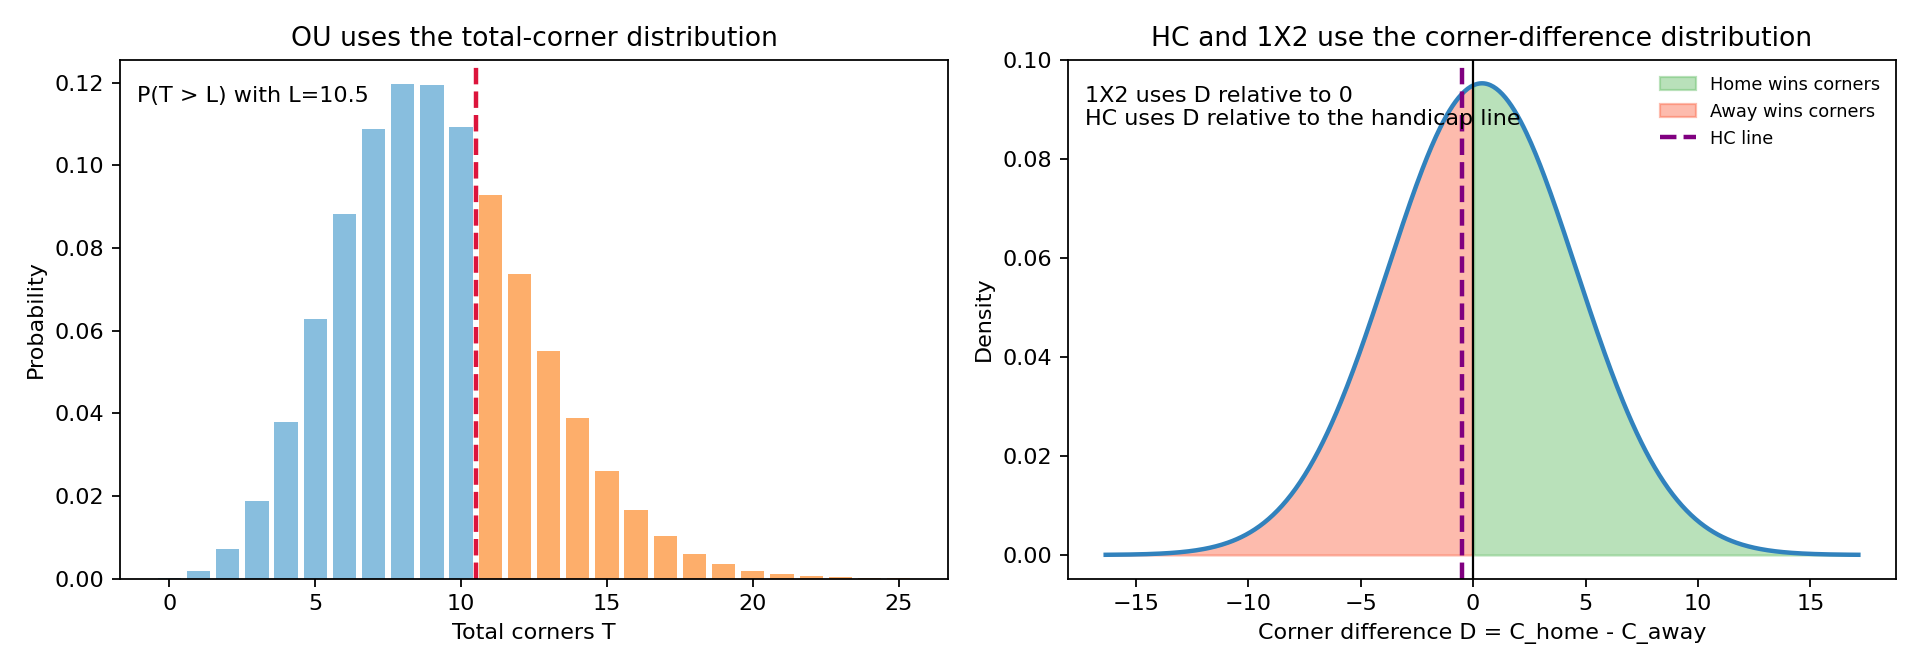
\includegraphics[width=0.92\textwidth]{../outputs/kelly_backtest/probability_construction.png}
\caption{How the model turns Q1 moments into market probabilities: OU uses the total-corner distribution, while HC and 1X2 use the corner-difference distribution.}
\end{figure}

For a decimal-odds bet with model win probability \(p\) and quoted odds \(o\), the unit-stake expected value is:
\[
\text{EV}=p\cdot o-1.
\]
That is the quantity used for filtering.

The raw model probabilities are then calibrated on partition A with per-side isotonic calibration, and the most aggressive positive-EV tails are shrunk back toward no-vig market probabilities when the model looks too confident. The final quantity used for selection is \texttt{ev\_tail}, not the uncalibrated EV.

Under the current default settings, the selection rule is:
\begin{itemize}
    \item bet 1X2 only if \(\text{EV} > 0.03\);
    \item bet HC only if \(\text{EV} > 0.023\);
    \item bet OU only if \(\text{EV} > 0.035\).
\end{itemize}

These thresholds are now tuned on partition A only, not on partition B. I ran a small grid on A alone:
\[
\text{1X2} \in \{0.02, 0.025, 0.03, 0.035, 0.04\},
\]
\[
\text{HC} \in \{0.018, 0.02, 0.023, 0.025, 0.028, 0.03\},
\]
\[
\text{OU} \in \{0.02, 0.025, 0.03, 0.035\}.
\]
Within that grid, \((0.03,\,0.023,\,0.035)\) was chosen as the final tuple. It is still selected on A only, but unlike the stricter \(0.035\) cut on 1X2, it keeps a non-zero 1X2 book alive. That is useful for portfolio construction: keeping some exposure across different market types helps avoid concentrating the whole book in only HC and OU, to reduce portfolio risk according to the portfolio optimization principles.

On clean partition B, this produces:
\begin{itemize}
    \item \(850\) selections in total;
    \item \(261\) from 1X2;
    \item \(456\) from HC;
    \item \(133\) from OU.
\end{itemize}

I am not betting every positive-EV line. I am only betting selections that clear the market-specific thresholds after calibration and tail shrink. The reason is practical: the smallest positive-EV bets are exactly where the model tends to be most optimistic, so it is better to give up some volume and keep the average edge cleaner.

\bigskip

\noindent \textbf{Question 3. ``Define Stake as the amount that you bet, calculate PnL as the Profit and Loss and RoI as PnL/Stake for each selection. (i) Calculate the overall PnL and RoI. (ii) Plot the cumulative PnL and EV as a function of time in days. (iii) Plot the 2-week rolling PnL and EV average.''}

\noindent \textbf{Answer.} For stake sizing, I use Kelly rather than flat staking. Kelly links bet size to estimated edge and current bankroll. More importantly, it comes from maximising expected log wealth rather than raw expected cash profit. That matters because log wealth strongly penalises paths that drive the bankroll close to zero.

For one bet with win probability \(p\), decimal odds \(o\), and stake fraction \(f\), the one-step expected log return is
\[
g(f)=p\log \left(1+f(o-1)\right)+(1-p)\log(1-f).
\]
The first-order condition gives the full Kelly fraction
\[
f^{*}=\frac{po-1}{o-1}.
\]
So Kelly is the fraction implied by maximising expected log growth. Compared with a plain EV rule, the log objective is much harsher on strategies that risk wiping out capital, because \(\log(B)\to -\infty\) as bankroll \(B\to 0\).

I test three stake policies:
\begin{itemize}
    \item \(100\%\) Kelly: \(f=f^{*}\);
    \item \(50\%\) Kelly: \(f=0.5f^{*}\);
    \item \(25\%\) Kelly: \(f=0.25f^{*}\).
\end{itemize}

The bankroll rules in this section are fixed as:
\begin{itemize}
    \item initial bankroll \(=100\) USD;
    \item fee rate \(=3\%\);
    \item minimum fee \(=0.1\) USD per bet;
    \item maximum single-bet stake \(=5000\) USD;
    \item bankroll cannot go below zero;
    \item once bankroll hits zero, betting stops.
\end{itemize}

The stopping rule is bankruptcy, not ``EV hits zero''. EV can move around from bet to bet, but the simulated path only ends when the bankroll itself reaches zero.

So for one candidate bet at time \(t\), the executable stake is
\[
s_t=\min(B_t\cdot f,\; 5000),
\]
where \(B_t\) is the current bankroll. The fee is
\[
\text{fee}_t=\max(0.03s_t,\;0.1).
\]
If several bets share the same kickoff time, the code rescales them so that the total cash outlay
\[
\sum_t (s_t+\text{fee}_t)
\]
does not exceed the bankroll available before that kickoff block.

For one realised bet with decimal odds \(o_t\), stake \(s_t\), fee \(\text{fee}_t\), and outcome \(w_t\in\{0,1\}\),
\[
\text{PnL}_t=
\begin{cases}
s_t(o_t-1)-\text{fee}_t, & \text{if } w_t=1,\\
-s_t-\text{fee}_t, & \text{if } w_t=0.
\end{cases}
\]
Overall PnL and turnover RoI are:
\[
\text{Total PnL}=\sum_t \text{PnL}_t,
\qquad
\text{RoI}=\frac{\sum_t \text{PnL}_t}{\sum_t s_t}.
\]

Under these exact bankroll constraints on partition B, the results are:
\begin{center}
\begin{tabular}{lccccc}
\toprule
Strategy & Total PnL & Ending Bankroll & Turnover RoI & Max Drawdown & Sharpe-style Proxy \\
\midrule
100\% Kelly & \(+1{,}299{,}009.53\) & \(1{,}299{,}109.53\) & \(35.03\%\) & \(-88.35\%\) & \(5.19\) \\
50\% Kelly & \(+1{,}246{,}238.09\) & \(1{,}246{,}338.09\) & \(36.91\%\) & \(-44.17\%\) & \(5.32\) \\
25\% Kelly & \(+1{,}062{,}903.30\) & \(1{,}063{,}003.30\) & \(38.11\%\) & \(-22.09\%\) & \(7.81\) \\
\bottomrule
\end{tabular}
\end{center}

None of the three Kelly paths went bust in this realised sample, but every path would have stopped immediately if bankroll had hit zero. Full Kelly still has extremely severe drawdowns. The most balanced line here is \(25\%\) Kelly: lower terminal PnL than full Kelly, but the highest turnover RoI, by far the mildest drawdown, and the best simple Sharpe-style proxy based on daily bankroll returns. That is why I would prefer \(25\%\) Kelly in practice. The point is not to maximise the paper terminal value at all costs. The point is to maximise risk-adjusted return.

For the time-series plots below, I use the \(25\%\) Kelly path because it is the practical choice from the table above. The cumulative EV line is the running sum of expected net PnL, where each bet contributes stake \(\times\) edge minus fee. The rolling plot then takes the daily realised and expected PnL series and averages them over a moving 14-day window.

\begin{figure}[htbp]
\centering
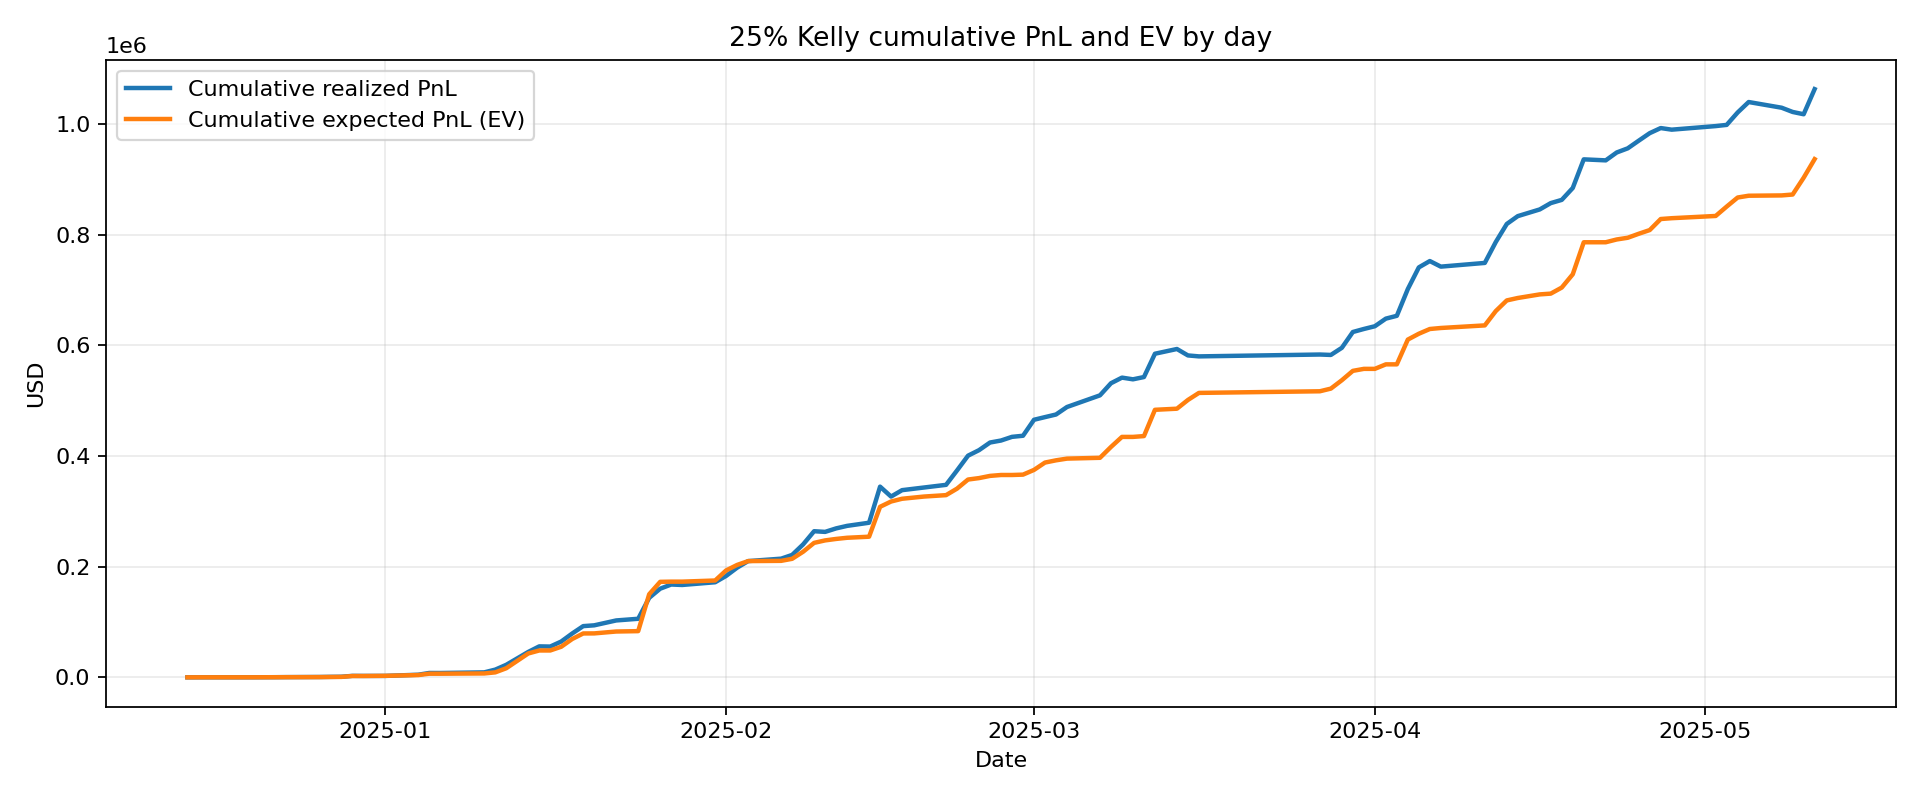
\includegraphics[width=0.84\textwidth]{../outputs/kelly_backtest/kelly_25_cumulative_pnl_ev.png}
\caption{25\% Kelly cumulative realised PnL and cumulative EV by day. }
\end{figure}

\begin{figure}[htbp]
\centering
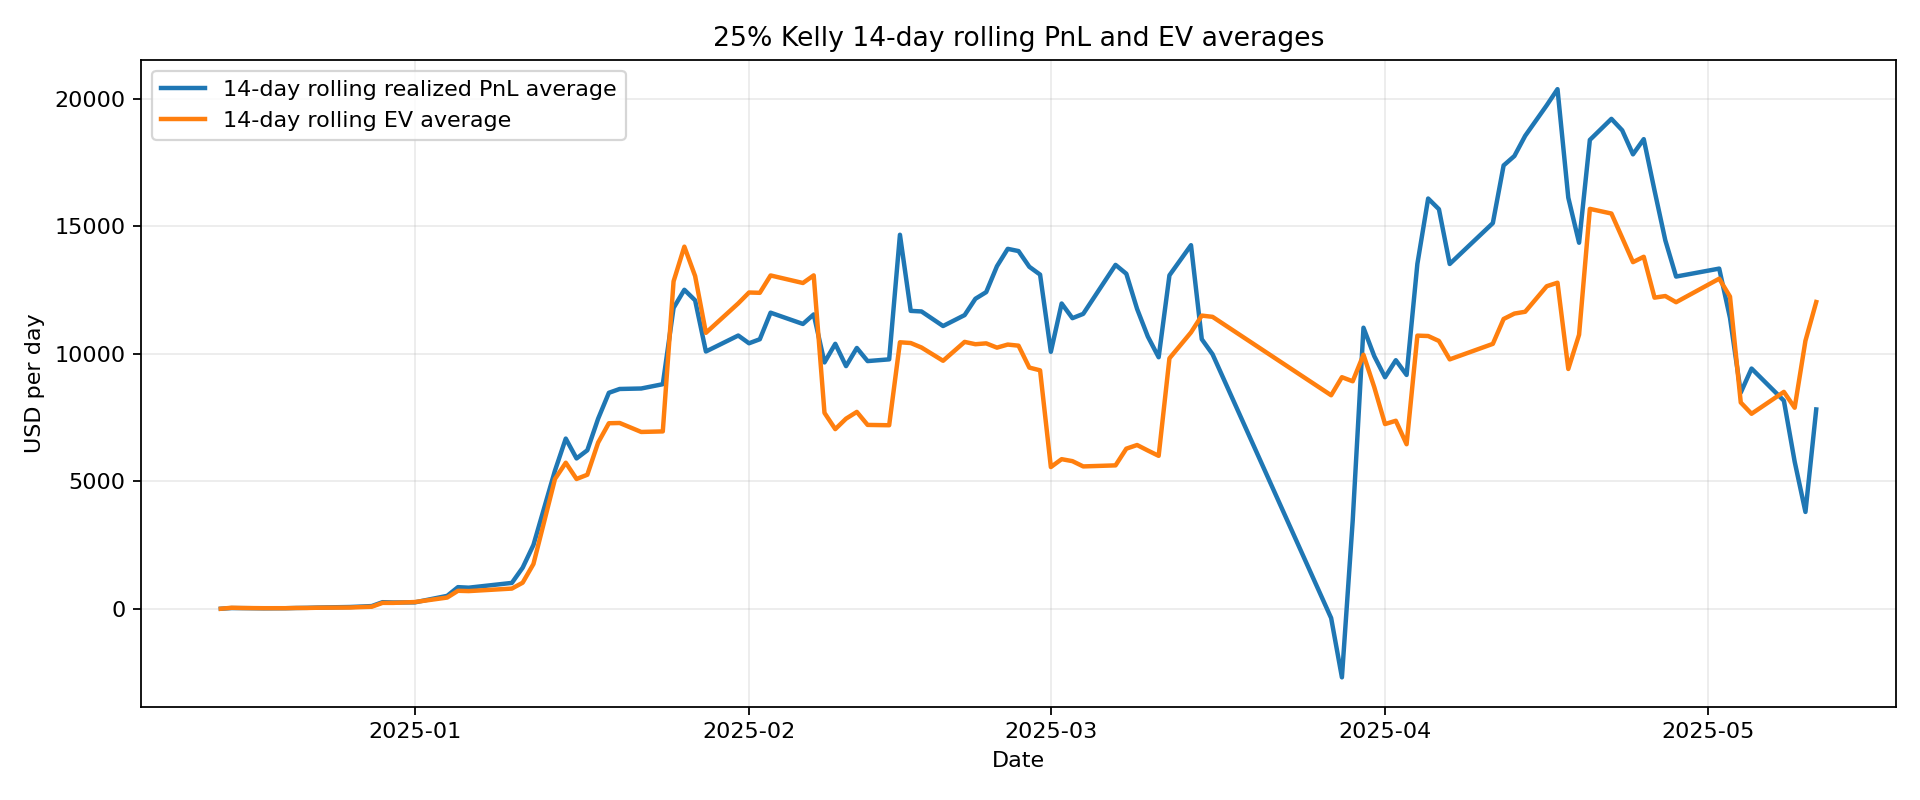
\includegraphics[width=0.84\textwidth]{../outputs/kelly_backtest/kelly_25_rolling_pnl_ev.png}
\caption{25\% Kelly 14-day rolling realised PnL average and 14-day rolling EV average. }
\end{figure}

\begin{figure}[htbp]
\centering
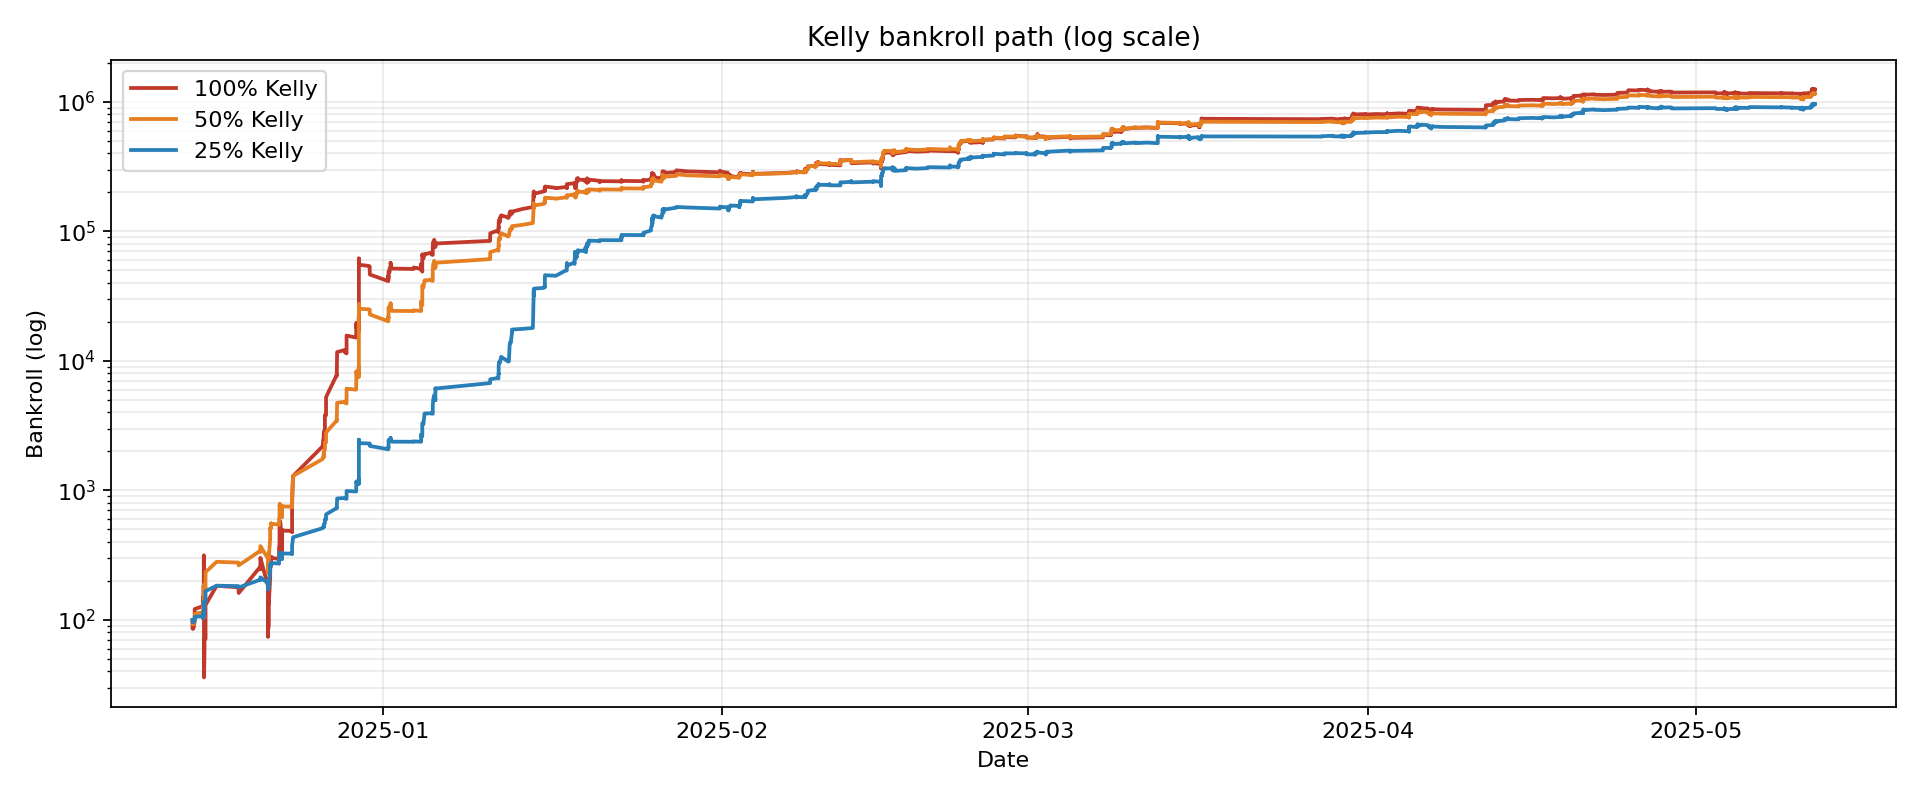
\includegraphics[width=0.84\textwidth]{../outputs/kelly_backtest/bankroll_paths_log.png}
\caption{Kelly bankroll paths on a log scale for 100\%, 50\%, and 25\% Kelly. This keeps the cross-strategy comparison visible alongside the 25\% Kelly time-series plots.}
\end{figure}

\bigskip

\noindent \textbf{Question 4. ``Do you think that your assumed EV is an accurate representation of your real edge? (Hint: Run a Monte Carlo simulation)''}

\noindent \textbf{Answer.} No. The assumed EV is a model output, not a ground truth edge. Kelly changes the stake size, but it does not repair probability miscalibration by itself. If the probability model is shifted, overconfident, or unstable, the real edge can be much smaller than the paper EV, and it can even turn negative.

To test this, I run a Monte Carlo simulation on the selected bets. For each selected bet \(i\), I treat the calibrated tail probability \(p_i\) as the Bernoulli win probability, simulate the bet outcome many times, and sum the simulated PnL across the whole portfolio. Repeating that gives a distribution for total PnL under the model's own assumptions.

I first simulate it and plot the empirical distribution. It looks roughly normal mainly because there are many bets, and total PnL is the sum of many small independent or near-independent random payoffs. So the normal shape is an outcome of the central limit effect.

If the model's EV were perfectly calibrated, the realised PnL would sit in a fairly ordinary part of that simulated distribution. If the realised PnL kept landing near the extreme lower tail, that would mean the model is overstating its edge.

The probability model behind the Kelly sizing was checked earlier with Monte Carlo on the selected partition-B bets:
\begin{itemize}
    \item actual total PnL \(=+303.49\);
    \item Monte Carlo median PnL \(=+249.57\);
    \item Monte Carlo 5th to 95th percentile range \(=[+181.92,\; +319.40]\);
    \item actual percentile \(=90\)th.
\end{itemize}

The realised outcome sits high in the model distribution, but that should be read carefully. A \(90\)th-percentile outcome does \emph{not} automatically mean the model understated its true edge. The safer interpretation is that this realised path was favourable relative to the model median. In other words, the backtest did well, but part of that success is still ordinary upper-tail luck. To claim that the model is systematically conservative, I would need to see the same pattern repeated across multiple independent periods, not just one partition-B run.

What is encouraging is more specific than that. The realised PnL is high, but it is not absurdly far outside the model range, and the selected book is concentrated in the cleaner HC and OU bets after calibration and tail shrink. So the simulation does not suggest a wildly misspecified model. But from a risk point of view, the main lesson is still about the downside: how bad can the portfolio look if the edge is weaker than the fitted model says?

That is why I treat Monte Carlo here mainly as a risk tool, not a victory lap. The useful outputs are the left tail, the stress scenarios, and how quickly the edge shrinks once the probabilities are perturbed. The question is not ``did this run make money?'' The question is ``how fragile is the portfolio if the model is even slightly wrong?''

To make the stress-test idea more concrete, I also plot one pessimistic scenario. In that scenario, I cut the model edge by shrinking each selected probability about \(27\%\) toward the no-vig market probability:
\[
p_{\text{stress}} = p_{\text{market}} + 0.73\left(p_{\text{tail}} - p_{\text{market}}\right).
\]
Under that stressed probability set, the Monte Carlo median falls to \(+182.43\), which sits around the 5th percentile of the original model distribution. This is the key risk message: a fairly modest haircut to the probabilities already moves the portfolio from ``comfortably above the model median'' to something that looks like a lower-tail outcome under the original assumptions. So even though the realised path was strong, the edge is still sensitive.

The more serious failure mode is distribution shift. If the home and away means drift, if the variance layer becomes too narrow, if the tails are mis-specified, or if the bookmaker market adapts, then the realised win rate can fall below the model probability. In that case Kelly can lose money fast because the stake is a direct function of estimated edge.

That is why stress testing matters. Reasonable stress tests here are:
\begin{itemize}
    \item shrink model probabilities toward market-implied probabilities;
    \item push the mean predictions away from their fitted values;
    \item widen or narrow the variance inputs;
    \item raise fees or lower the maximum bet size;
    \item remove the highest-EV tail and see how much of the PnL survives.
\end{itemize}
If the strategy only works under the exact fitted distribution, then the edge is too fragile.

There is also a market risk: if a bookmaker detects an advantage player, it can lower the bet cap, delay acceptance, or restrict the account entirely. In that case the theoretical Kelly fraction is no longer deployable, so realised growth can be much lower than the paper path even if the raw EV estimate is correct.

This is another reason that I prefer showing \(25\%\) and \(50\%\) Kelly alongside full Kelly rather than trusting full Kelly blindly. If the EV estimate is even slightly too high, full Kelly overreacts immediately. Fractional Kelly gives more room for model error.

\begin{figure}[htbp]
\centering
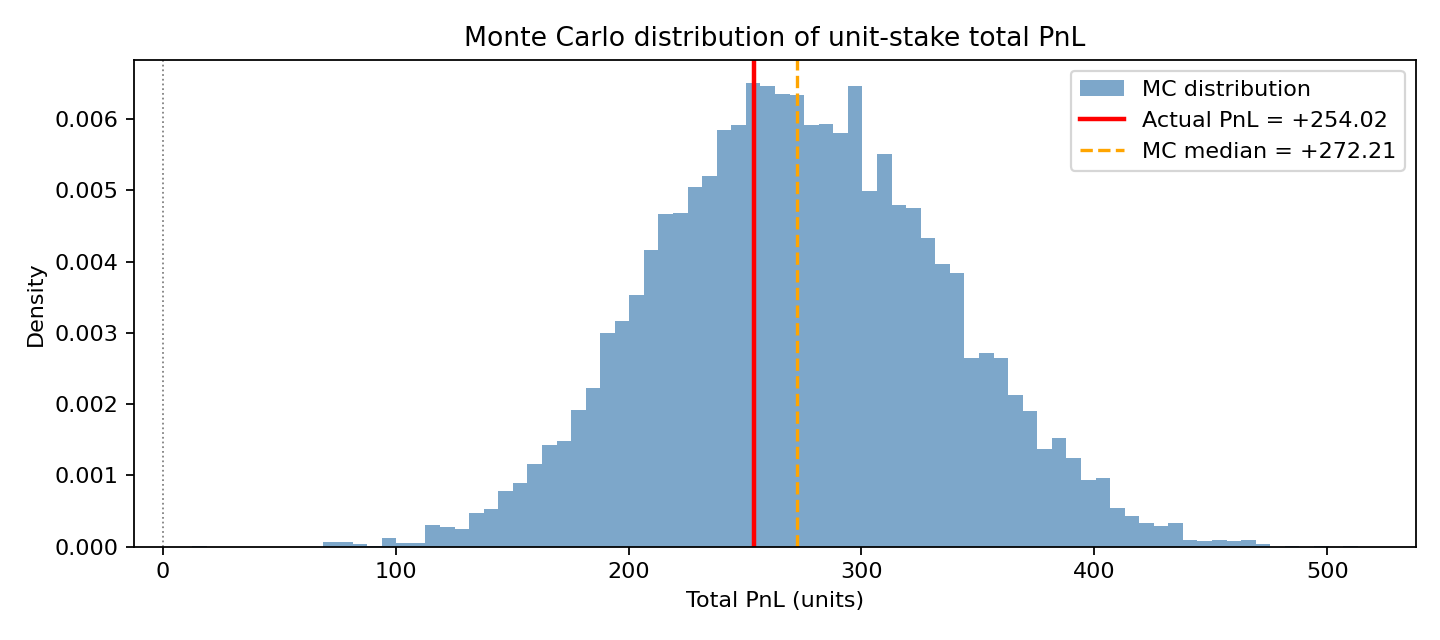
\includegraphics[width=0.82\textwidth]{../outputs/kelly_backtest/selection_edge_monte_carlo.png}
\caption{Monte Carlo distribution of unit-stake total PnL for the selected partition-B bets, with one stressed scenario overlaid. The stressed line uses an approximately 27\% shrink toward market-implied probabilities so that the stressed median lands near the 5th percentile of the original model distribution.}
\end{figure}

\end{document}
